\section{Future work}

%Predicting evolution?

%In writing this dissertation, I have been both plagued and delighted to have many %ideas that would perfectly encapsulate certain elements of historical contingency. 
%The issue is time; one is in graduate school for a finite number of years, with the goal of minimizing that time. 
%As such, to avoid a 10-year PhD, I will relegate these ideas to this section. 
%I think it is inevitable when writing a dissertation to have many ideas that would be \textit{perfect}, if only you had a little more time.
%In my experience, it is impossible to conduct the experments and write up a dissertation without coming up with the \textit{perfect} experiments to 
%At the very least, this has been the case for me; I have a plethora of ideas but not time to conduct the experiments and write them up. 
%Thus here I will splurge and metaphorically ``stake my claim''. 

We will first consider the obvious extensions to this work. 
Foremost, while the chapters of this dissertation dive deep into the role that history plays in evolution, I have analyzed only three experimental setups (two related environments in Avida and a simple one-dimensional integral landscape).
We clearly need to expand this work to other types of organisms and environments. 
My long-term hope is for adventurous and determined wet lab evolutionary biologists to conduct more studies in this vein. 
However, I have barely begun to scratch the surface of digital evolution models.
As such, here I discuss two axes we should vary: the digital evolution model and the task or environment within it.
We can also vary the parameters of the system (e.g., the mutation rate, population size, etc), which I discuss in detail below. 

There exist dozens of mature digital evolution, evolutionary computation, and similar software models in use today. 
One particular avenue of exploration is to see how potentiation dynamics change between these different models. 
For example, Chapters \ref{chap:learning_case_studies} and \ref{chap:learning_distributions} study the evolution of associative learning in Avida using a path following task. 
Would the potentiation of path-following associative learning in Markov Brains \citep{hintzeMarkovBrainsTechnical2017} or PushGP \citep{spectorGeneticProgrammingAutoconstructive2002} follow similar trends to those observed in Avida? 
The solutions would certainly look quite different, but future experiments are needed to empirically compare the potentiation dynamics.

Even if we limit ourselves to studies within Avida, potentiation dynamics may drastically differ across environments. 
Would we see large increases in potentiation of optimal plasticity in the plasticity environment from Chapter \ref{chap:consequences_of_plasticity} or in the potentiation of the logic trait EQU in the classic ``logic 9'' environment \citep{ofriaAvidaSoftwarePlatform2004a}?
Comparison across these environments is favorable: we could use roughly the same instruction set (barring environment-specific instructions), population size, mutation operators, etc. 
I find it likely, however, that potentiation dynamics would still differ.
As discussed in Chapter \ref{chap:learning_distributions}, I hypothesize that potentiation is influenced by the optimization needed \textit{after} the first versions of a behavior appear, which is possible, for example, with suboptimal plasticity. 
In the ``logic 9'' environment, some logic tasks are building blocks of others. 
It is possible their potentiation is thus highly correlated, but it is also possible that the potentiation for a simple task actually \textit{decreases} when it appears, as it actualizes in a way that makes it likely to be lost as the more complex tasks evolve. 

%Chapters \ref{chap:consequences_of_plasticity} through \ref{chap:learning_distributions} all use Avida, yet there remain infinitely many experimental tweaks that could change the results in interesting ways. 
%These range from the simplest tweaks, such as seeing how potentiation dynamics change as we vary mutation rate, to broad-scale comparisons of how potentiation dynamics change across domains: associative learning (Chapter \ref{chap:learning_case_studies} and \ref{chap:learning_distributions}), phenotypic plasticity (Chapter \ref{chap:consequences_of_plasticity}), and the classic ``logic 9'' \citep{ofriaAvidaSoftwarePlatform2004a} environment may have drastically different potentiation dynamics. 
%Though adaptive momentum is a unique dynamics, I have shown that systems as simple as evolving integers can display intricate potentiation dynamics. 

%Below, at the risk becoming esoteric, I detail more specific ideas that have arisen during the creation of this thesis. 
Below I detail more specific ideas that have arisen during the creation of this thesis. 

\subsection{On the multiplicative nature of potentiation}

Chapters \ref{chap:learning_case_studies} and \ref{chap:learning_distributions} identify ``potentiating mutations'' that caused the largest increases in potentiation for a given lineage. 
However, this is only one interpretation of the ``largest increase'' in potentiation, focusing on the absolute percentage point change. 
%We are successfully identifying the mutation that causes the \textit{absolute} largest change in potentiation. 
We could, however, shift to a \textit{relative} view of potentiation. 
%Let us illustrate the difference in these methods with an example. 
To illustrate the difference in these two values, imagine we have two mutations. 
The first mutation increases potentiation from 10\% to 40\%, while the second increases potentiation from 40\% to 80\%. 
Under our current framing, the second mutation is our largest potentiating mutation, as it increases potentiation by 40 percentage points (compared to 30 for the first mutation). 
However, an alternate framing is that the first mutation quadrupled the probability of evolving our focal trait, while the second mutation only doubled the probability. 

\begin{figure}[h!]
\begin{center}
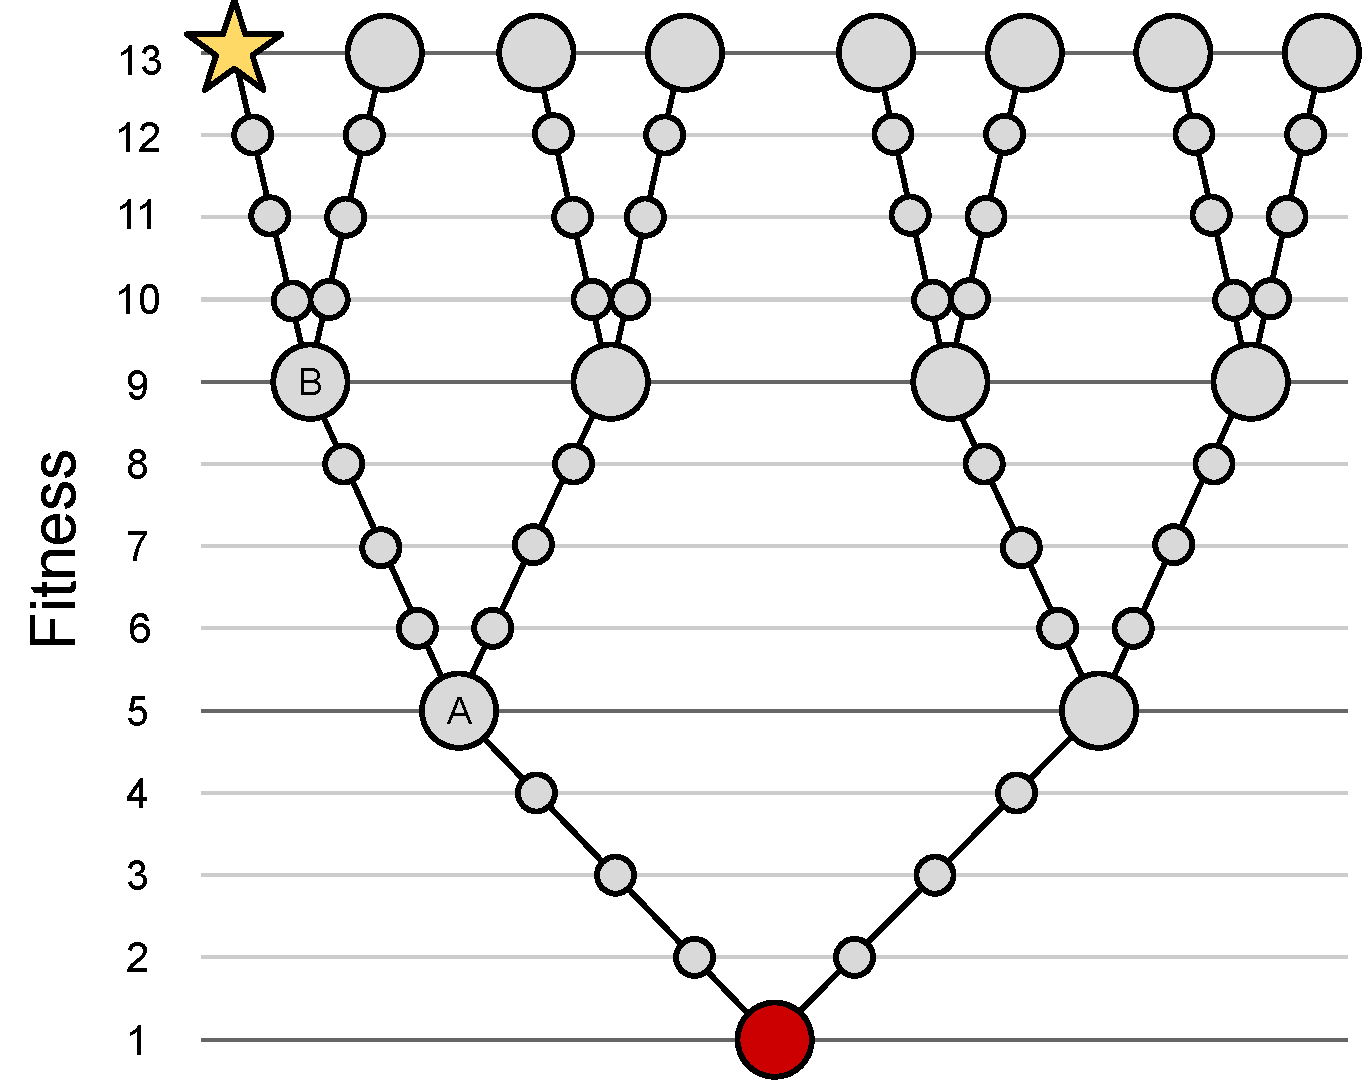
\includegraphics[width=0.65\textwidth]{06_conclusion/media/bst.pdf}
\end{center}
\caption{ 
A hypothetical fitness landscape in the form of a binary tree. 
Each node represents a particular genotype, and edges represent available mutations. 
Branch points, which have two higher-fitness neighbors, are shown larger than other nodes. 
The root node is shown in red, and two nodes are marked (A and B) for the in-text example. 
We can consider potentiation relative to the star, which can be reached with a series of mutations that use the left option at each branch point. 
}\label{fig:conclusion_binary_tree}
\end{figure}

To begin contemplating the ramifications of using absolute vs relative potentiation change, we can consider the simple fitness landscape in Figure \ref{fig:conclusion_binary_tree}.
If we assume a scenario with a low mutation rate and strong selection pressure, since fitness increases from the root node to the leaves, evolutionary theory dictates that all populations should evolve to a leaf node. 
%Fitness increases as we move from the root node to the leaves, so we expect all populations to evolve to a leaf node, assuming selection is strong enough. 
%Additionally, the population will reach two branching points over the course of evolution. 
Depending on the starting node, the population can encounter branching nodes over the course of evolution. 
Since each branching node has two neighboring nodes with higher yet equal fitness, we expect the population to go down each branch with 50\% probability. 
Here we consider the potentiation of the population evolving to reach the star node. 
In this example, potentiation for the star node from nodes between node B and the star are all approximately 100\%. 
Potentiation at the node B is expected to be 50\%, as the population will either evolve down the left or right branch. 
Similarly, potentiation is expected to be 25\% at node A and 12.5\% at the root node.
Thus, in terms of absolute potentiation differences along a trajectory from the root to the target node, potentiation will increase most moving from node B to the left at a 50\% increase. 
However, if we instead look at relative increases, moving off of the root, node A, and node B are all the same, doubling potentiation. 
This difference is demonstrated in Figure \ref{fig:conclusion_diff_types}

\begin{figure}[h!]
\begin{center}
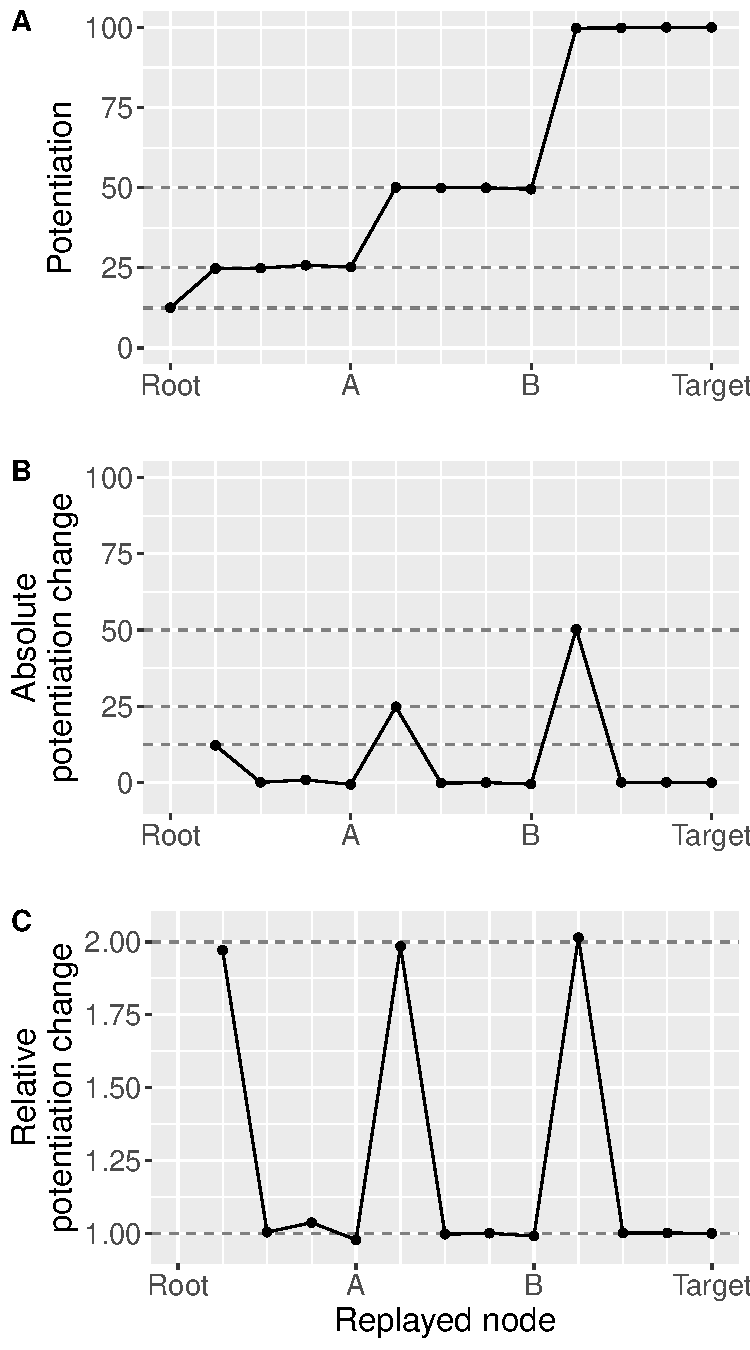
\includegraphics[width=0.58\textwidth]{06_conclusion/media/combined_plot_10k.pdf}
\end{center}
\caption{ 
Empirically measured potentiation of nodes from the fitness landscape in Figure \ref{fig:conclusion_binary_tree}. 
Subplot A shows potentiation for each node on the left side of the tree. 
Potentiation for a node is calculated as the percentage of replicates (out of 10,000) started with a full population of 100 organisms on that node that evolve to the target node after 500 generations of roulette selection.
Subplot B shows the absolute potentiation change when moving to each node, calculated as the difference between potentiation measured from the current position and the previous position. 
Subplot C shows the relative potentiation change, calculated as the potentiation measured at the current position divided by potentiation measured at the previous position.
}\label{fig:conclusion_diff_types}
\end{figure}

Considering these differences as absolute or relative are both valid approaches, in the same way that other measures such as epistasis can be measured either additively or multiplicatively. 
%In many cases we will be limited by the practical limitations of collecting enough data in order to measure potentiation with sufficient precision.
In Chapters \ref{chap:learning_case_studies} and \ref{chap:learning_distributions} I took an absolute approach as I wanted to analyze the overall potentiation of associative learning and how it changed. 
While the ``decision points'' encountered by evolution are interesting, they were not my main focus. 
What did prove relevant, however,is that because those experiments were conducted in Avida, I was limited to the resolution of my data.
I strained the computation resources available in order to do 50 replays for each potentiation measurement, meaning that I had a base resolution of $2\%$ intervals, before even considering noise.
A 5\% to 10\% increase can be significant and impactful, but the number of replicates needed to determine that difference with a high degree of statistical confidence were computationally infeasible. 
Future work should consider both approaches however, as large relative increases in potentiation might happen much earlier in the population's history and might provide additional insight. 

\subsection{Understanding factors that influence potentiation}

In Chapter \ref{chap:learning_case_studies}, I detailed the inner mechanics of the digital organisms and how the potentiating mutations paved the way for the evolution of learning. 
However, which dynamics factor into potentiation are still poorly understood. 
For example, my initial hypothesis was that most potentiating mutations would be deleterious or neutral, as beneficial mutations are likely to get selected and thus unlikely to influence the overall probability that the focal trait evolves. 
Chapter \ref{chap:learning_distributions} provided strong counter evidence, with 49 of 50 potentiating mutations being either beneficial or having no significant fitness effect. 
This raises the question: what other factors are at play in potentiation?

Three factors I want to draw attention to are the size of the mutational neighborhood, the mutation rate, and the size of the population.
Combined with the topography of the fitness landscape, these factors dictate the likelihood that a given mutation will appear. 
Specifically, as the number of neighbors increases, the mutation rate decreases, or the population size decreases, it becomes less likely that any given mutation will ever occur. 
As such, even the mutation with the highest possible fitness can be potentiating, as there is a chance \textit{it never appears} and thus selection cannot act upon it.
Additionally, even if a highly beneficial mutation appears, there is always the chance that it is lost to genetic drift.
Future studies should examine how varying each of these parameters in isolation changes the potentiation dynamics. 
In designing the experiment in Chapter \ref{chap:learning_case_studies}, I chose to use Avida partially because I was unsure how much complexity was needed to observe interesting potentiation changes. 
Chapter \ref{chap:adaptive_momentum} has demonstrated that this complexity is not required. 
While future work should observe potentiation in other complex systems, potentiation should also be studied in the simplest possible systems to conduct controlled studies like the ones mentioned here. 


\subsection{Improving evolutionary computation}

This dissertation is focused on improving our understanding of evolution as a process and the refinement of techniques to be applied back to wet lab studies. 
However, these techniques and ideas can also be applied to the problem-solving field of evolutionary computation (EC).
In order to improve efficiency and problem-solving ability, EC practitioners are constantly refining their evolving systems. 
Even beyond the initial design phase, most systems have a collection of parameters and operators to fine-tune the system for the particular task at hand. 
Optimizing the design decisions and parameter values of these systems is a continuous effort in EC research. 

How might a better understanding of historical contingency and potentiation improve our understanding in these systems? 
Let us imagine that we want to test the effects of adding new mutational operators to our EC system. 
A proper first step would be to run a two treatment experiment: one batch of experiments that have access to these new operators and a control treatment that does not. 
With enough replicates, we should see if our changes improve the problem solving success of our system. 
Indeed, we could dive further and test these new operators in isolation or in combination, to disentangle which operators improve our success. 

To consider the benefit of adopting a history-based mindset, we must switch from asking \textit{if} these new mutational operators improve our problem solving success to asking \textit{how} the new operators improve our evolutionary search.
We can, and often do, make inferences about what events might have been critical to a replicate's success. 
For example, we might identify a gene duplication event occurring shortly before the focal trait evolves.
However, only by experimentally testing the effect of accumulated history can we verify which specific events were pivotal in the population's ultimate success and which were mere coincidence. 
In our example, the gene duplication mentioned above might have helped, but it also may have followed another mutation whose importance is harder to detect. 
It is this interplay of dynamics that we aim to clarify. 
By leveraging these techniques, we may be able to nail down interactions between constituent parts, such as our mutation operators, that are beneficial and that we want to encourage via our design choices and parameters settings. 

However, with this increased analytic power comes an increase in computational requirements. 
Techniques such as replay experiments have the potential to deliver critical insights into EC systems, but they are too computationally expensive to conduct regularly. 
As such, future work should aim to identify cases where these techniques are most useful, so practitioners can leverage them when they are the correct tool for the job. 

%\subsection{Quantifying tradeoffs}

\subsection{Quantifying evolvability}

Generally, analytic replay experiments have focused on the potentiation of beneficial traits. 
This leads to a simple observation: if the focal trait is beneficial, an increase in its potentiation is likely to correspond to an increase in the long-term fitness of the lineage, depending on the alternative trajectories that could have been taken.
Though we lack an agreed upon definition of evolvability \citep{pigliucciEvolvabilityEvolvable2008}, here I use the definition of \citet{payneCausesEvolvabilityTheir2019}: ``the ability of a biological system to produce phenotypic variation that is both heritable and adaptive''.
Thus, I argue that an increase in average long-term fitness constitutes an increase in evolvability.

I am not the first to combine the ideas of evolvability and historical contingency. 
\citet{woodsSecondorderSelectionEvolvability2011} were among the first to leverage analytic replay experiments, and they used these replays to test the long-term evolvability of two clades of \textit{E. coli}.
In the original replicate, the clade that eventually won had lower fitness at the time of sampling. 
Replay experiments started from that original point demonstrated that the ``eventual winner'' clade consistently evolved higher fitness despite its lower initial fitness -- it was more \textit{evolvable}.

\begin{figure}[h!]
\begin{center}
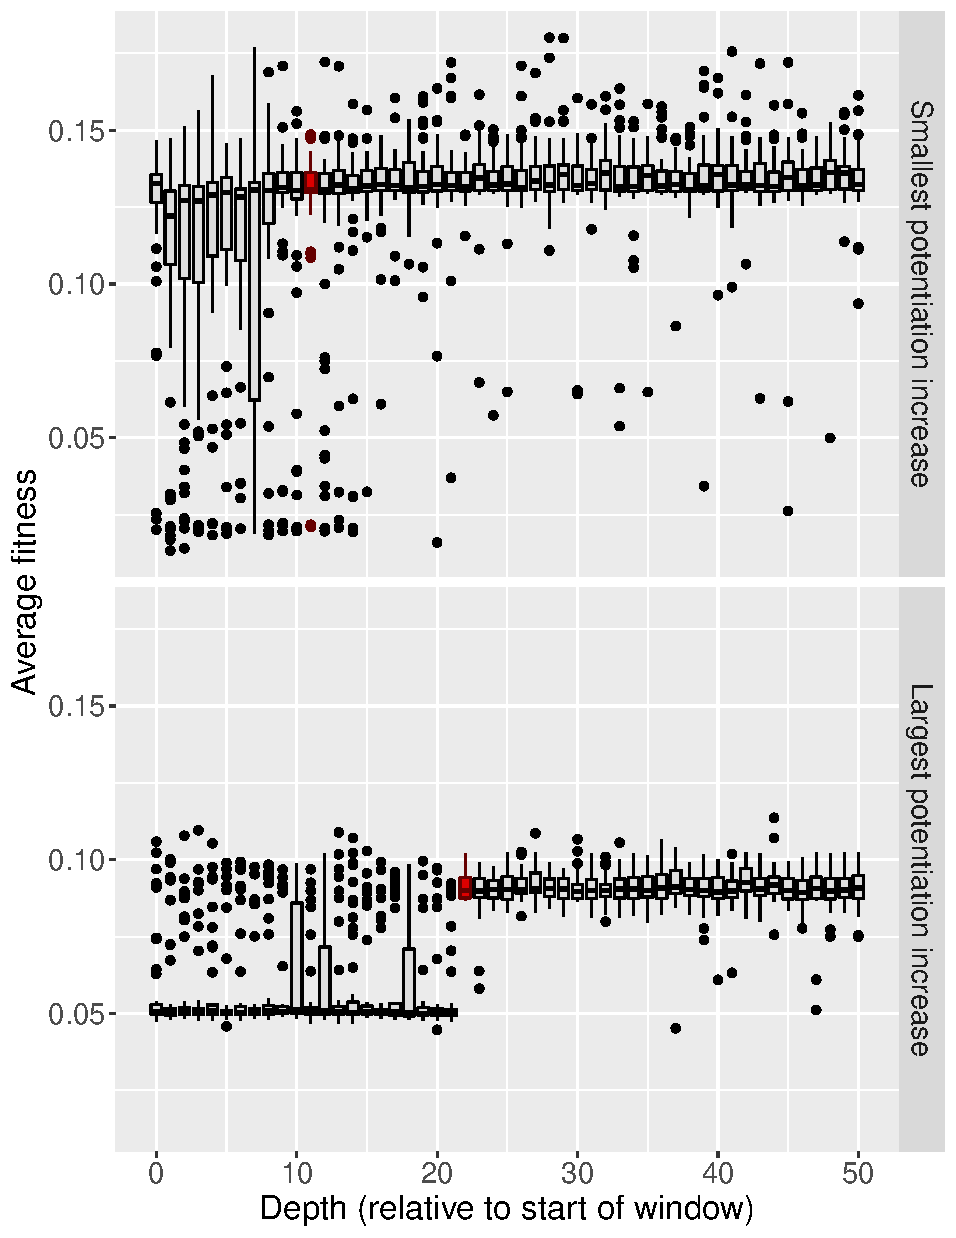
\includegraphics[width=0.75\textwidth]{06_conclusion/media/evolvability.pdf}
\end{center}
\caption{ 
Two examples of evolvability data from the targeted replays of Chapter \ref{chap:learning_distributions}. 
A boxplot is shown for each depth replayed in the targeted replays, corresponding to the average fitness at the end of each of the 50 replicates replayed from that depth. 
The red boxplot shows the potentiating step. 
Two lineages are shown, one with a small potentiation increase (20 percentage points) and little change in long-term fitness, and another with a large potentiation increase (88 percentage points) and a stark increase in long-term fitness with the potentiating step. 
}\label{fig:conclusion_evolvability}
\end{figure}


In conducting multiple replay experiments, I have realized that these systems are ripe for further studies in evolvability. 
We must first consider the concept of ``evolvability-enhancing muations'' as introduced by \citep{wagnerEvolvabilityenhancingMutationsFitness2023}. 
Evolvability-enhancing mutations are defined as mutations whose one-step mutational neighborhood has a higher average fitness than the one-step neighborhood of the wild type.
As noted by the author, we could also define these evolvability-enhancing mutations using a two-step, three-step, or larger mutational neighborhood. 
Increasing the range of the mutational neighborhood would overcome issues such as evolvability-enhancing mutations that lead to local fitness peaks, limiting long-term fitness.

Unfortunately, performing a N-step mutant analysis becomes intractable on most fitness landscapes for, at most, $N > 2$.
Thankfully, we can make a simplification: what if we only consider the mutational trajectories that are most likely? 
This is exactly what replay experiments do; each replay replicate samples the fitness landscape that is reachable from the starting condition in a given amount of time.
While we are only sampling a fraction of the possible trajectories, the sample should be representative of what will evolve from the starting condition. 


Finally, conducting these studies requires \textit{little to no additional work}.
If a replay experiment is conducted to observe the potentiation dynamics of a lineage for a particular trait, the only additional step is to also evaluate fitness at the end of each replay replicate. 
In Chapter \ref{chap:learning_distributions}, I had to quantify fitness in order to determine if the replay replicates evolved learning. 
As such, \textit{these data already contain information on evolvability}.
Unfortunately, a full analysis of these data are out of scope for this dissertation. 
A preliminary examination is shown in Figure \ref{fig:conclusion_evolvability}, exhibiting the long-term fitness of the replays from two lineages. 
One lineage, which had only a 20 percentage point increase in potentiation, sees little change in the long-term fitness at the potentiating step. 
The second lineage, which had the largest single-step potentiation increase (88 percentage points), sees a substantial increase in long-term fitness. 
When we consider these results through the lens of potentiation, we see that the higher-fitness trajectories were always present, potentiating mutations are simply biasing evolution toward these high-fitness areas, and thus, increasing evolvability. 
Future work should further explore these dynamics; my hypothesis is that the increase in potentiation and the increase in long-term fitness should be correlated in systems where the potentiation trait being measured represents a highly beneficial adaptation. 